\documentclass{standalone}
\usepackage{tikz}
\usepackage{pgfplots}
%\pgfplotsset{compat=newest}
\usetikzlibrary{calc}
\usepackage{ifthen}
\newcommand\mycolor{white}
\usetikzlibrary{matrix}
\usetikzlibrary{patterns}

\begin{document}
    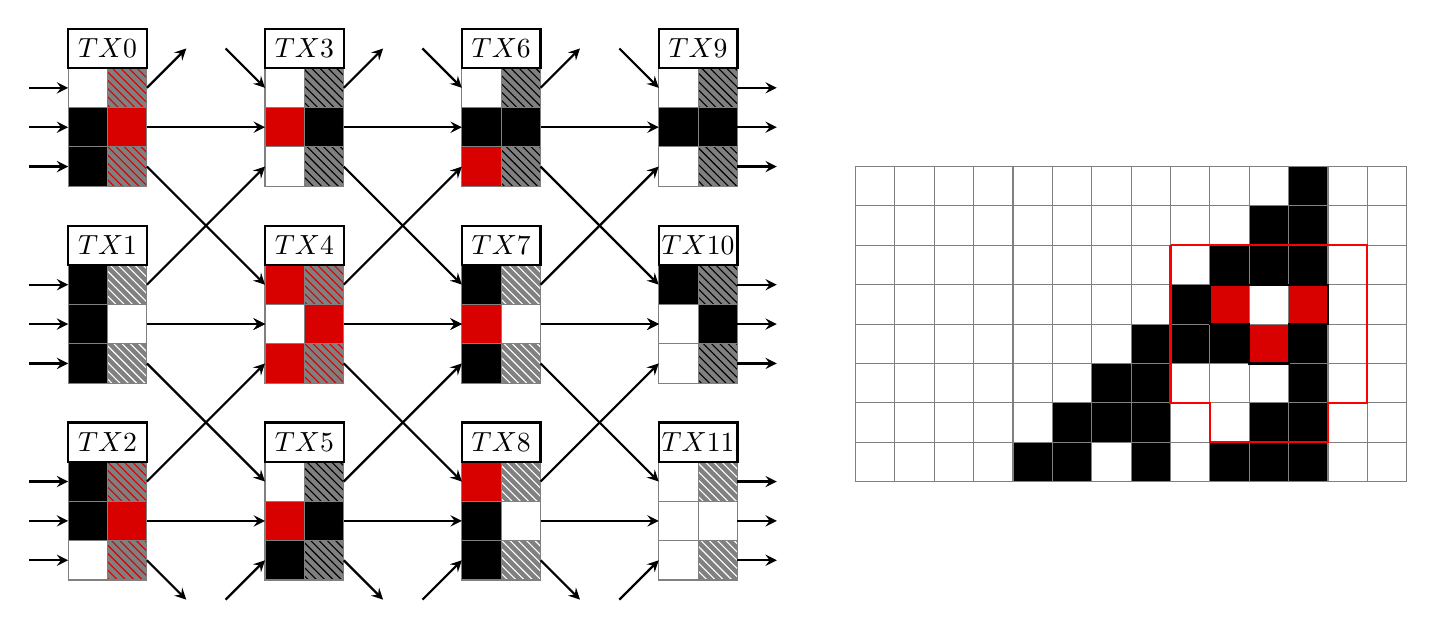
\begin{tikzpicture}[
        X/.style={draw=gray, minimum size=5mm, outer sep=0pt},
        B/.style={X, fill},
        C/.style={X, fill=black!15!red},
        D/.style={X, preaction={fill, gray}, pattern=north west lines, pattern color=black!15!red},
        E/.style={X, preaction={fill, gray}, pattern=north west lines, pattern color=black},
        F/.style={X, preaction={fill, gray}, pattern=north west lines, pattern color=white},
%    D/.style={X, preaction={fill, black!15!red}, pattern=north west lines},
%    E/.style={X, preaction={fill, black}, pattern=north west lines, pattern color=white},
%    F/.style={X, preaction={fill, white}, pattern=north west lines},
        mymatrix/.style={matrix of nodes, row
            sep=-\pgflinewidth,
            column sep=-\pgflinewidth, nodes={X}, nodes in
        empty cells}
    ]

    \def\h{0.5}
    \def\dy{2.5}
    \def\dx{2.5}
    \def\dmatr{13}
    \def\xmax{3}

    \matrix at (0,\dy)[mymatrix]{
        &|[D]|\\
        |[B]|&|[C]|\\
        |[B]|&|[D]|\\
    };

    \matrix at (0,0)[mymatrix]{
        |[B]|&|[F]|\\
        |[B]|&\\
        |[B]|&|[F]|\\
    };

    \matrix at (0,-\dy)[mymatrix]{
        |[B]|&|[D]|\\
        |[B]|&|[C]|\\
        &|[D]|\\
    };

    \matrix at (\dx,\dy)[mymatrix]{
        &|[E]|\\
        |[C]|&|[B]|\\
        &|[E]|\\
    };

    \matrix at (\dx,0)[mymatrix]{
        |[C]|&|[D]|\\
        &|[C]|\\
        |[C]|&|[D]|\\
    };

    \matrix at (\dx,-\dy)[mymatrix]{
        &|[E]|\\
        |[C]|&|[B]|\\
        |[B]|&|[E]|\\
    };

    \matrix at (2*\dx,\dy)[mymatrix]{
        &|[E]|\\
        |[B]|&|[B]|\\
        |[C]|&|[E]|\\
    };

    \matrix at (2*\dx,0)[mymatrix]{
        |[B]|&|[F]|\\
        |[C]|&\\
        |[B]|&|[F]|\\
    };

    \matrix at (2*\dx,-\dy)[mymatrix]{
        |[C]|&|[F]|\\
        |[B]|&\\
        |[B]|&|[F]|\\
    };

    \matrix at (3*\dx,\dy)[mymatrix]{
        &|[E]|\\
        |[B]|&|[B]|\\
        &|[E]|\\
    };

    \matrix at (3*\dx,0)[mymatrix]{
        |[B]|&|[E]|\\
        &|[B]|\\
        &|[E]|\\
    };

    \matrix at (3*\dx,-\dy)[mymatrix]{
        &|[F]|\\
        &\\
        &|[F]|\\
    };

    \foreach \y in {-1,0,1}{
        \foreach \z in {-1,0,1}{
            \draw[thick, ->, >=stealth] (-2*\h,{\dy*\y+\z*\h}) -- (-\h,{\dy*\y+\z*\h});
            \draw[thick, ->, >=stealth] (\xmax*\dx+\h,{\dy*\y+\z*\h}) -- (\xmax*\dx+2*\h,{\dy*\y+\z*\h});
        }
        \foreach \x in {0,...,\xmax}{
            \pgfmathsetmacro\ind{int(3*\x + 1 - \y)}
            \draw[thick] ({\dx*\x-\h}, \dy*\y+1.5*\h) rectangle ({\dx*\x+\h}, \dy*\y+2.5*\h);
            \node at ({\dx*\x}, \dy*\y+2*\h) {$TX\ind$};
        }
    }
    \pgfmathsetmacro\xmaxm{int(\xmax-1)}
    \foreach \x in {0,...,\xmaxm}{
        \foreach \y in {-1,0,1}{
            \draw[thick, ->, >=stealth] (\dx*\x+\h,\dy*\y) -- ({\dx*(\x+1)-\h},\dy*\y);
            \draw[thick, ->, >=stealth] (\dx*\x+\h,\h*\y) -- ({\dx*(\x+1)-\h},{(-\h+\dy)*\y});
            \draw[thick, ->, >=stealth] (\dx*\x+\h,{(-\h+\dy)*\y}) -- ({\dx*(\x+1)-\h},\h*\y);
        }
        \draw[thick, ->, >=stealth] (\h+\dx*\x,\dy+\h) -- (2*\h+\dx*\x,\dy+2*\h);
        \draw[thick, ->, >=stealth] (\h+\dx*\x,-\dy-\h) -- (2*\h+\dx*\x,-\dy-2*\h);
        \draw[thick, ->, >=stealth] ({-2*\h+\dx*(\x+1)},\dy+2*\h) -- ({-\h+\dx*(\x+1)},\dy+\h);
        \draw[thick, ->, >=stealth] ({-2*\h+\dx*(\x+1)},-\dy-2*\h) -- ({-\h+\dx*(\x+1)},-\dy-\h);
    }

    \matrix at (\dmatr,0) [mymatrix]{
        &&&&&&&&&&&|[B]|&&\\
        &&&&&&&&&&|[B]|&|[B]|&&\\
        &&&&&&&&&|[B]|&|[B]|&|[B]|&&\\
        &&&&&&&&|[B]|&|[C]|&&|[C]|&&\\
        &&&&&&&|[B]|&|[B]|&|[B]|&|[C]|&|[B]|&&\\
        &&&&&&|[B]|&|[B]|&&&&|[B]|&&\\
        &&&&&|[B]|&|[B]|&|[B]|&&&|[B]|&|[B]|&&\\
        &&&&|[B]|&|[B]|&&|[B]|&&|[B]|&|[B]|&|[B]|&&\\
    };

    \draw[thick] (\dmatr+2*\h,\h) -- (\dmatr+5*\h,\h) -- 
    (\dmatr+5*\h,0) -- (\dmatr+4*\h,0) -- (\dmatr+4*\h,-\h) -- 
    (\dmatr+3*\h,-\h) -- (\dmatr+3*\h, 0) -- (\dmatr+2*\h, 0) -- (\dmatr+2*\h, \h);

    \draw[thick,red] (\dmatr+\h,2*\h) -- (\dmatr+6*\h,2*\h) -- (\dmatr+6*\h,
    {(1-\xmax)*\h}) --(\dmatr + 5*\h, {(1-\xmax)*\h}) -- 
    (\dmatr+5*\h,-\xmax*\h) -- (\dmatr+2*\h,-\xmax*\h) 
    -- (\dmatr+2*\h,{(1-\xmax)*\h}) -- (\dmatr+\h, {(1-\xmax)*\h}) -- (\dmatr+\h,2*\h);
\end{tikzpicture}
\end{document}
